\documentclass{report}
\usepackage[margin=0.75in]{geometry}
\usepackage{ccfonts}
\usepackage{graphicx}
\begin{document}
    \newcommand{\BASIC}[0]{{\sc Basic816}}
    \newcommand{\keyword}[1]{{\tt {#1}}}
    \newcommand{\param}[1]{{\tt <{#1}>}}
    \title{The \BASIC\  Language Manual}
    \author{PJW}
    \date{19 March 2021}
    \maketitle

    \section*{About \BASIC}

    \BASIC\ is an implementation of the BASIC programming language for the Western Design Center's 65816 microprocessor.
    It is focused on providing a simple BASIC interpreter for the C256 Foenix computer designed by Stefany Allaire.
    \BASIC\ has a few design goals and even a couple of anti-goals:

    \begin{itemize}
        \item It should provide a retro-computing feel.
        \item It should be simple to use and easy to learn.
        \item It should provide essential access to storage and the C256's abilities.
        \item It should be expandable, allowing advanced users to customize it or extend it.
        \item It should be a clean-room implementation, unencumbered by copy-right. 
        \item It need not be the fastest programming language available.
        \item It need provide all the advancements in programming languages developed since the 1980s.
    \end{itemize}

    As such, \BASIC\ is a fairly traditional, tokenized, line-number based implementation of BASIC, similar to those
    implementation of BASIC on the 8-bit computers of the 1970s and 1980s.

    \section*{Screen Editing}

    BASIC816 for the C256 includes a simple screen editor.
    To enter a program, just type the lines, being sure to press the return key at the end of each line.
    The interpreter will not attempt to process the line until you press return, and the text it will process
    is whatever text is on the line of the screen where your cursor is.
    If you need to edit a line that's on the screen, you can use the cursor keys to move to the line and make your change.
    A few other special keys are supported:

    \begin{itemize}
        \item[Arrow Keys] The arrow keys will move the cursor on the screen in a natural fashion.
        \item[Backspace] The backspace key deletes the character to the left of the cursor.
        \item[Delete] The delete key deletes the character under the cursor.
        \item[Insert] The insert key inserts a space at the cursor (pushing the character that was under the cursor to the right).    
    \end{itemize}

    Although not an edit key, the SysRq key is currently assigned as a ``programmer's key'' and will interrupt
    the currently running BASIC program and open the monitor. It should work for any program (even machine language), so
    long as the keyboard interrupt logic has not been intercepted. Likewise, the Scroll Lock key will pause any screen
    output from the interpreter while it is on. This includes output from a program that is producing a lot of text and
    even program listings.

    \section*{Data Types}

    \BASIC\ supports three data types:

    \begin{itemize}
        \item[Integer]  The integers in \BASIC\ are 32-bit signed integers and may have values from $-2,147,483,648$ to $2,147,483,647$.
                        Examples of integers are $0$, $1$, $42$, $-1$, $-128$.

        \item[Float]    The floating point numbers in \BASIC\ are 32-bit floating points using the IEEE-754 format,
                        which uses an 8-bit exponent, a 23-bit mantissa, and a single sign bit. Given a mantissa of $m$ and an exponent of
                        $x$, the value of the floating point number is $m \times 2^x$. Floating point numbers in \BASIC\ are represented in one
                        of two ways, either as a decimal number or using scientific notation:
                        \verb+1.0+, \verb+-23.45+, \verb+1.0e-03+, \verb+3.0e08+.

        \item[String]   Text data are stored in strings. A string may be entered into a \BASIC\ program by enclosing it in double quote marks.
                        Strings are represented internally as null-terminated ASCII strings, that is, there is no length data on the string,
                        the end of which is marked by a 0 byte.
                        Strings may be up to 65536 bytes in length.
                        
        \item[Array]    Arrays allow multiple data items to be stored under a single name and accessed by an index.
                        Two types of arrays are supported: arrays of integer and arrays of strings.
                        Arrays may be just one-dimensional, using a single number as index, or they may be multi-dimensional,
                        where each element has a unique combination of numbers serving as an index.
    \end{itemize}

    Unlike many implementations of BASIC, \BASIC\ treats floating point numbers differently from integer numbers.
    Operations on integer values or integer variables are performed using integer code and result in an integer value.
    Operations on floating point values or variables are performed using floating point code and result in a floating point value.
    On the C256, integer code generally uses the integer math coprocessor, while floating point code uses the floating point math
    coprocessor.
    Integers and floating point numbers can be converted between each other. If an operation is expecting a floating point value,
    the interpreter will attempt to convert an integer to floating point. If it is expecting an integer, it will attempt to
    convert a floating point value to an integer.
    One caveat to converting between integers and floating point numbers is that \BASIC\ integers have 32-bits of precision, but
    the floating point numbers have only 23 bits of precision for the mantissa.

    \subsection*{Literal Values}

    Integers, floats, and strings may be entered directly into programs as literal values.
    Strings are designated with double quote marks, but there is no character escape
    syntax as in other languages. If you need to enter a character you cannot type,
    you will have to use the \verb+CHR$+ function. Integers may be entered as a sequence
    of digits with an optional minus sign at the start. The default base for integers
    is decimal, but hexadecimal numbers may be entered with the \verb+&H+ prefix.
    Floating point numbers may only be entered using decimal digits and must include a
    decimal point.

    \begin{itemize}
        \item \verb+"Hello, world!"+
        \item \verb+12345+
        \item \verb+-562+
        \item \verb+&HFFD2+
    \end{itemize}

    \section*{Variables}

    A \BASIC\ program can assign data to variables using the \keyword{LET} statement or an implicit \keyword{LET} statement.
    Variables need not be declared before use, with the exception of array variables, which must be declared through the
    \keyword{DIM} statement.

    Variable names may be up to eight characters long. The first character must be an alphabetic character from A through Z.
    Subsequent characters of the name may be A--Z, 0--9, or the underscore character (\_). The type of the variable is indicated
    by a character at the end of the variable name. Integer variables are indicated by the percent sign (\%), and string
    variables are indicated by the dollar sign (\$).
    Floating point variables have no type character.
    These type designations must be used in all references to the variable and may
    be considered as part of the name. This means that a program can have six different variables with the same ``name'' but different
    types (e.g. \verb+A+, \verb+A%+, \verb+A$+, \verb+A()+, \verb+A%()+, and \verb+A$()+).

    \section*{Expressions}

    An expression is a sequence of values, operators, and function calls which will have some data value as a {\em result}.
    An expression may have a numeric (integer) result or a text (string) result.

    Operators are common mathematical symbols which will perform some sort of computation on two values. These are the usual
    sort of thing: addition, subtraction, multiplication, division, and so on. Operators are typically evaluated left to right,
    but have an operator precedence which can alter the order of execution. For instance multiplication operators are evaluated
    before addition. This precendence can be altered by using parentheses to enclose a sub-expression that should be evaluated
    as a unit.

    \begin{table}[!htb]
        \begin{center}
            \begin{tabular}{|l|l|} \hline
                Operators & Purpose \\ \hline\hline
                \verb+^+ & Exponent \\ \hline
                \verb+*+, \verb+/+, \verb+MOD+ & Multiply, Divide, modulo \\ \hline
                \verb-+-, \verb+-+ & Addition, Subtraction \\ \hline
                \verb+<+, \verb+>+, \verb+=+ , \verb+<=+, \verb+>=+, \verb+<>+ & Comparison operators \\ \hline
                \verb+NOT+ & Bitwise Negation \\ \hline
                \verb+AND+ & Bitwise AND \\ \hline
                \verb+OR+ & Bitwise OR \\ \hline
            \end{tabular}
            \caption{Operators in order of descending precedence.}
        \end{center}
    \end{table}

    NOTE: the division operator performs a floating point division always results in a floating point value,
    even if the numerator and denominator are divisible.

    \section*{Commands}

    Commands in \BASIC\ are keywords which triggers some action but which may only be used at the interactive prompt.
    Commands may not be used within a \BASIC\ program.

    \subsection*{\keyword{CONT}}

    Continue execution of the current program from the point immediately after the \keyword{STOP} statement that was executed.
    It is an error to use this command if the current program was not interrupted by the \keyword{STOP} command or if there
    is no current program.

    \subsection*{\keyword{DIR}}

    Print a listing of the files on the current file device.

    \subsection*{\keyword{DEL} \param{filename}}

    Delete a file from a file device.

    \subsection*{\keyword{NEW}}

    \verb+NEW+ clears all of \BASIC's memory. All program and variable data are erased, and a new program may be entered.

    \subsection*{\keyword{{LIST [\param{start}] [- \param{end}]}}}

    \verb+LIST+ types a program listing to the console screen. It accepts two optional line-numbers to limit the listing.
    The first line number specifies the smallest line number to list; if it is not specified, there is no lower limit.
    The second line number specifies the largest line number to list; if it is not specified, there is no upper limit.

    \subsection*{\keyword{LOAD} \param{filename}}

    Load the BASIC program with the given file name.

    \subsection*{\keyword{SAVE} \param{filename}}

    Save the BASIC program to storage with the given file name.
    The file must not already exist.
    
    \subsection*{\keyword{RUN}}

    Starts execution of the program from the first line of the code.

    \section*{Statements}

    Statements are keywords which trigger some action and may be used either at the interactive prompt or within a program.
    A \BASIC\ program can be seen as a series of lines, each of which must have one or more statements on it.
    If a line has more than one statement, each statement is separated from the next by a colon (:).

    \subsection*{\keyword{BLOAD} \param{filename} [, \param{destination}]}

    Loads a binary file into memory starting at the specified \param{destination} address in memory. If there is no
    provided \param{destination}, the file format loaded must have its own destination address embedded within it.
    Currently, only the \keyword{PGX} format is supported, but others may be supported in future.

    \subsection*{\keyword{BRUN} \param{filename}}

    Load the binary file specified into memory and attempt to execute it.
    The file must be in an executable format, which means that it must contain its own destination address
    and information on how to start it. Currently, only the \keyword{PGX} format is supported, but others
    may be supported in the future.

    \subsection*{\keyword{BSAVE} \param{filename}, \param{start}, \param{end}}

    Save the data in memory from address \param{start} to address \param{end} (inclusive) to a binary file.
    The file must not already exist.

    \subsection*{\keyword{CLR}}

    Erases all variable definitions. Any variable that was defined prior to the use of \keyword{CLR} will be undefined.
    Also all data stored directly or indirectly through variables will be returned to free memory. This is similar to
    \keyword{NEW}, except that the program may be running and is left intact.

    \subsection*{\keyword{CLS}}

    Clears the text screen and moves the cursor to the home position.

    \subsection*{\keyword{CALL \param{address}[, \param{a}[, \param{x}[, \param{y}]]]}}

    Call a machine language subroutine at \param{address}. If the subroutine returns at all to the caller, it
    must return using the \keyword{RTL} instruction. Values may be provided for the \keyword{A}, \keyword{X}, and
    \keyword{Y} registers and may be 16-bit values.

    \subsection*{\keyword{DATA \param{value}[, ...]}}

    Provide numeric or string data in the program which may be retrieved into a variable using the \keyword{READ} statement.

    \subsection*{\keyword{DEL} \param{filename}}

    Delete a file from the storage device.

    \subsection*{\keyword{DIM \param{variable}(\param{size}[, ...])}}

    Declare an array named \param{variable}.
    The array can have many dimensions, each with the size provided.
    An array can have up to 127 dimensions, and the size can be up to 256, but in practice the entire block of memory
    consumed by the array cannot exceed 65,536 bytes (including the ``book keeping'' memory allocated to keep track of the array
    (which is at most 256 bytes).

    \subsection*{\keyword{END}}

    Stops execution of the program. The only way to restart execution after \keyword{END} has been
    executed is to use the \keyword{RUN} command.

    \subsection*{\keyword{FOR} \param{variable} = \param{initial} \keyword{TO} \param{target} [\keyword{STEP} \param{increment}]}

    The \keyword{FOR} statement marks the beginning of a loop that will repeat a specified number of times.
    It starts by assigning an \param{initial} value to a \param{variable} and executing the following statement until
    the matching \keyword{NEXT} statement is encountered. It will then either add 1 to \param{variable} or
    \param{increment}, if provided. So long as \param{variable} is not \param{target}, the statements between the
    \keyword{FOR} and \keyword{NEXT} will be executed.

    \subsection*{\keyword{GET} \param{variable}}

    Waits for the user to press a key, the assigns the character of that key to the string \param{variable} provided.

    \subsection*{\keyword{GOTO} \param{line number}}

    Continue execution with the first statement on the line with the given \param{line number}.
    It is an error to \keyword{GOTO} a \param{line number} that does not exist in the program.

    \subsection*{\keyword{GOSUB} \param{line number}}

    Call a subroutine starting at the line with the given \param{line number}.
    A subsequent \keyword{RETURN} statement will return the program to the statement
    following the \keyword{GOSUB}.
    It is an error to \keyword{GOSUB} a \param{line number} that does not exist in the program.

    \subsection*{\keyword{IF} \param{expr} \keyword{THEN} \param{line}}

    Evaluates \param{expr} and examines the result.
    If the result is not zero, execution continues with the first statement on the line with number \param{line}.
    Otherwise, execution continues with the next statement after the \keyword{IF}.

    Note: This statement will be receiving considerable improvements in subsequent versions of \BASIC.

    \subsection*{\keyword{INPUT} [ \param{message}; ] \param{variable}}

    If a literal string message is provided, print the message followed by a question mark.
    If no message is provided, just print a question mark.
    In either case, wait for the user to type a line of input on the keyboard and
    put the value typed into the provided variable.

    NOTE: Currently, this statement supports only string values and variables.

    \subsection*{\keyword{NEXT}}

    Close the matching \keyword{FOR} loop.

    \subsection*{\keyword{POKE} \param{address}, \param{value}}

    Write the 8-bit \param{value} to the memory location at \param{address}.
    It is an error to try to write a value that requires more than 8-bits.

    \subsection*{\keyword{POKEW} \param{address}, \param{value}}

    Write the 16-bit \param{value} to the memory location at \param{address}.
    The low byte of \param{value} will be written to \param{address}, and
    the high byte of \param{value} will be written to the following byte in memory.
    It is an error to try to write a value that requires more than 16-bits.    

    \subsection*{\keyword{POKEL} \param{address}, \param{value}}

    Write the 24-bit \param{value} to the memory location at \param{address}.
    The low byte of \param{value} will be written to \param{address}, and
    the middle byte of \param{value} will be written to the following byte in memory,
    and the high byte of \param{value} will be written to the next byte in memory.
    It is an error to try to write a value that requires more than 24-bits.  

    \subsection*{\keyword{PRINT} [\param{value} [,/;]] ...}

    Write the textual representation of \param{value} to the screen.
    If more than one \param{value} is provided, they must be separated by either a comma (,)
    or a semicolon (;).
    If a comma is used, the two items will be separated by a TAB.
    If a semicolon is used, the two items will be printed one after the other.
    A \keyword{PRINT} statement will print a carriage return as the last thing, unless the
    statement is ended with a semicolon.

    \subsection*{\keyword{REM} \param{comment}}

    Inserts a comment into the \BASIC\ program. All characters after the \keyword{REM} until
    end of the line will be ignored.

    \subsection*{\keyword{READ} \param{variable}[, ...]}

    Read one of more values out of the \keyword{DATA} statements in the program into
    \param{variable}.
    The data read must have a compatible type to the variable.
    Each variable read will advance a data cursor forward one data element.
    If a \keyword{READ} is executed when the cursor has reached the end of the data
    elements, it is an error.

    \subsection*{\keyword{RENAME} \param{path}, \param{filename}}

    Renames the existing file at \param{path} to \param{filename}.

    \subsection*{\keyword{RESTORE}}

    Resets the data cursor to the first data element of the first \keyword{DATA} statement.

    \subsection*{\keyword{STOP}}

    Stops execution of the program in such a way that the user can restart it with the
    \keyword{CONT} command.

    \section*{Functions}

    \subsection*{\keyword{ABS(\param{value})}}

    Returns the absolute value of \param{value}.
    If the parameter is negative, it is converted to its positive equivalent
    (for instance, \verb+ABS(-5)+ will evaluate to \verb+5+).

    \subsection*{\keyword{ASC(\param{text})}}

    Returns the ASCII code for the first character of \param{text}.
    Example: \verb+ASC("A")+ returns \verb+65+.

    \subsection*{\keyword{CHR\$(\param{value})}}

    Returns the character corresponding to the ASCII code in \param{value}.
    Example: \verb+CHR$(65)+ returns \verb+"A"+.
    
    \subsection*{\keyword{COS(\param{value})}}

    Returns the cosine of \param{value}, which should be in radians.

    \subsection*{\keyword{DEC(\param{hex})}}

    Returns an integer that is conversion of the hexadecimal number in the string \param{hex}.
    Example: \verb+DEC("A0") + returns \verb+160+.

    \subsection*{\keyword{HEX\$(\param{value})}}

    Returns a string that is the hexadecimal representation of the integer value passed.
    Example: \verb+HEX$(160) + returns \verb+"A0"+.

    \subsection*{\keyword{INT(\param{value})}}

    Converts a floating point \param{value} to an integer by truncating the fractional part.
    The value returned is of integer type.

    \subsection*{\keyword{LEFT\$(\param{text}, \param{count})}}

    Returns the left-most \param{count} characters of the string \param{text}.

    Example: \verb+LEFT$("Hello", 3)+ returns \verb+"Hel"+.   

    \subsection*{\keyword{LN(\param{value})}}

    Returns the natural logarithm (base $e$) of \param{value}.

    \subsection*{\keyword{MID\$(\param{text}, \param{first}, \param{count})}}

    Returns a substring of the string \param{text}.
    The parameter \param{first} specifies the number of the first character to use, where
    a \verb+0+ is the number of the first character in the source string.
    The parameter \param{count} indicates how many characters should be returned.

    Example: \verb+MID$("Hello", 2, 3)+ returns \verb+"llo"+.

    \subsection*{\keyword{PEEK(\param{address})}}

    Returns the byte stored in memory at location \param{address}.

    \subsection*{\keyword{PEEKW(\param{address})}}

    Returns the 16-bit word stored in memory at location \param{address}.
    The low byte of the returned value is at \param{address}, and the
    high byte is at \verb-address + 1-.

    \subsection*{\keyword{PEEKL(\param{address})}}

    Returns the 24-bit word stored in memory at location \param{address}.
    The low byte of the returned value is at \param{address},
    the middle byte is at \verb-address + 1-, 
    and the high byte is at \verb-address + 2-.

    \subsection*{\keyword{RIGHT\$(\param{text}, \param{count})}}

    Returns the right-most \param{count} characters of the string \param{text}.

    Example: \verb+LEFT$("Hello", 3)+ returns \verb+"llo"+.

    \subsection*{\keyword{RND(\param{value})}}

    Returns a pseudo-random floating point number between 0.0 and 1.0.
    Note that the input value is not used and can be any number.
    
    \subsection*{\keyword{SGN(\param{value})}}

    Returns the sign of the number \param{value}.
    If the number is negative, the result is \verb+-1+,
    if the number is positive, the result is \verb+1+,
    and if the number is zero, the result is \verb+0+.

    Example: \verb+SGN(-25)+ returns \verb+-1+.

    \subsection*{\keyword{SIN(\param{value})}}

    Returns the sine of \param{value}, which should be in radians.

    \subsection*{\keyword{SPC(\param{value})}}

    Returns a string containing \param{value} spaces.
    
    Example: \verb+SPC(5)+ returns a string of five spaces.

    \subsection*{\keyword{STR\$(\param{value})}}

    Returns a string containing the decimal representation of the number \param{value}.
    
    Example: \verb+STR$(25)+ returns \verb+"25"+.

    \subsection*{\keyword{TAB(\param{value})}}

    Returns a string containing \param{value} TAB characters.
    
    Example: \verb+TAB(2)+ returns a string of two TABs.

    \subsection*{\keyword{TAN(\param{value})}}

    Returns the tangent of \param{value}, which should be in radians.

    \subsection*{\keyword{VAL(\param{text})}}

    Returns the numeric value represented by the string of decimal digits in \param{text}.
    
    Example: \verb+VAL("42")+ returns \verb+42+.

    \section*{C256 Specific Statements}

    \BASIC\ includes a number of statements to support features of the C256 Foenix.

    \subsection*{\keyword{BITMAP} \param{plane}, \param{visible}, \param{lut} [, \param{address}]}

    Controls the visibility of the bitmap display (the bitmap engine must be
    enabled with the \keyword{GRAPHICS} command). The parameter \param{visible}
    must be a number. If it is 0, the bitmap will be hidden. If it is any other
    value, it will be shown.

    The number of the color lookup table to use must be provided as \param{lut},
    which must be the number of one of the graphics color lookup tables.

    Optionally, an address may be provided for the first byte of the bitmap.
    This address must be in the video memory starting at 0xB00000.
    If no address is provided, the it will default to 0xB00000.

    \subsection*{\keyword{CLRBITMAP} \param{plane}}

    Sets all pixels in the bitmap to 0 (transparent).
    \param{plane} is the number of the bitmap plane (0 or 1).
    The bitmap must have been setup with the \keyword{BITMAP} statement before
    this statement can be used.

    \subsection*{\keyword{FILL} \param{plane}, \param{x0}, \param{y0}, \param{x1}, \param{y1}, \param{color}}

    Fill the rectangle with corners at $(x_0, y_0)$ to $(x_1, y_1)$ with the color
    specified by the \param{color} index number.
    \param{plane} is the number of the bitmap plane (0 or 1).
    The actual color displayed will depend on the RGB values provided for
    that index in the color lookup table currently used by the bitmap.
    The \keyword{BITMAP} statement must have been used before using
    this statement.

    \subsection*{\keyword{GRAPHICS} \param{mode}}

    Sets the graphics mode of the Vicky chip.
    This statement just sets the master control register of the Vicky chip to
    whatever value is provided in \param{mode}, which should be a number in the range 0--255.

    The bits of the master control register can be seen described in Table~\ref{vicky_mcr}.

    \begin{table}[!htb]
        \begin{center}
            \begin{tabular}{|l|l|l|} \hline
                Bit & Purpose \\ \hline\hline
                9 & Pixel Double: 0 = use base resolution, 1 = use half base resolution \\ \hline
                8 & Base Resolution: 0 = 640x480, 1 = 800x600 \\ \hline
                7 & Global disable: If set, this disables all Vicky output. \\ \hline
                6 & Gamma Correction: If set, this enables gamma correction. \\ \hline
                5 & Sprites: If set, this enables the sprite engine. \\ \hline
                4 & Tiles: If set, this enables the tile engine. \\ \hline
                3 & Bitmap: If set, this enables the bitmap engine. \\ \hline
                2 & Graphics: If set, this enables the graphics blocks. \\ \hline
                1 & Text Overlay: If set, text will be displayed over graphics. \\ \hline
                0 & Text: If set, this enables the text display engine. \\ \hline
            \end{tabular}
            \caption{Vicky Master Control Regiser}
            \label{vicky_mcr}
        \end{center}
    \end{table}

    One of the big changes with VICKY II is support of multiple display resolutions: 320x240,
    400x300, 640x480, 800x600. The resolution is set using bits 8 and 9 of the master control
    register. Bit 8 sets the base resolution by setting the display clock frequency, and bit 9
    turns on and off the pixel doubler. These resolution bits affect text as well as graphics
    rendering. So, choosing mode \verb+&h101+ will switch to a high resolution text mode with
    up to 100 characters per row (if the border is turned off).

    \begin{table}[!htb]
        \begin{center}
            \begin{tabular}{|l|l|l|} \hline
                Bit 9 & Bit 8 & Resolution \\ \hline\hline
                0 & 0 & 640x480 (default) \\ \hline
                0 & 1 & 800x600 \\ \hline
                1 & 0 & 320x240 \\ \hline
                1 & 1 & 400x300 \\ \hline
            \end{tabular}
            \caption{Vicky Display Resolutions}
            \label{vicky_res}
        \end{center}
    \end{table}    

    \subsection*{\keyword{LINE} \param{plane}, \param{x0}, \param{y0}, \param{x1}, \param{y1}, \param{color}}

    Draw a line on the bitmap display from positions $(x_0, y_0)$ to $(x_1, y_1)$ in the color
    specified by the \param{color} index number.
    \param{plane} is the number of the bitmap plane (0 or 1).
    The actual color displayed will depend on the RGB values provided for
    that index in the color lookup table currently used by the bitmap.
    The \keyword{BITMAP} statement must have been used before using
    this statement.

    \param{plane} is the number of the bitmap plane (0 or 1).

    The number of the color lookup table to use must also be provided as \param{color},
    which must be the number of one of the graphics color lookup tables.

    \subsection*{\keyword{LOCATE} \param{column}, \param{row}}

    Move the text cursor to the specified \keyword{column} and \keyword{row} on the text screen.
    Both arguments may be from 0 to 255, but no attempt is made to validate that the coordinates are
    valid for the current text mode.

    \subsection*{\keyword{MONITOR}}

    Enter the machine language monitor.

    \subsection*{\keyword{MEMCOPY} \param{source} \keyword{TO} \param{destination}}

    Request a copy of one block of memory to another block using the C256's DMA capabilities.
    In the C256, DMA transfers can work with two different memory topologies.
    A block of memory to be copied can be a linear (or ``1D'') block of contiguous bytes, or
    it can be a rectangular (or ``2D'') block of bytes, which can be a smaller region of a
    larger rectangular block. An example of this latter topology is when a program wants to
    copy a 32 pixel by 32 pixel block out of a 640 by 480 image.

    In order to specify the block topology, \param{source} and \param{destination} must
    use one of two forms:

    \begin{description}
        \item[\keyword{LINEAR} \param{address}, \param{length}]
            This structure specifies that the block is 1D or linear and starts at \param{address}
            and consists of \param{length} contiguous bytes. (See: Figure~\ref{memcopy_1d})
        
        \item[\keyword{RECT} \param{address}, \param{width}, \param{height}, \param{stride}]
            This structure specified that the block is a 2D or rectangular block.
            The block starts at \param{address} and is \param{width} bytes wide and
            \param{height} bytes high.
            The block is part of a potentially larger rectangular ``image'' that is
            \param{stride} bytes wide. (See: Figure~\ref{memcopy_2d})
    \end{description}

    \begin{figure}[htbp]
        \centering
        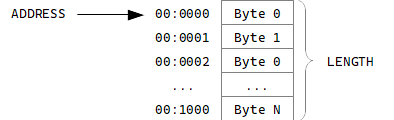
\includegraphics{MEMCOPY_LINEAR.png}
        \caption{A linear (1D) memory block}
        \label{memcopy_1d}
    \end{figure}

    \begin{figure}[htbp]
        \centering
        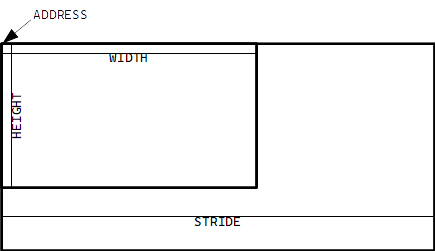
\includegraphics{MEMCOPY_RECT.png}
        \caption{A rectangular (2D) memory block}
        \label{memcopy_2d}
    \end{figure}

    Within certain limits, source and destination can use two different memory topologies,
    so the structures of source and destination do not need to match.
    An example where this
    might be useful is when a program loads a small icon file that is 32 by 32 pixels and
    then copies it to video RAM for display on a 640 by 480 screen:

    \begin{verbatim}
MEMCOPY LINEAR &h010000, 1024 TO RECT &hB00000,32,32,640
    \end{verbatim}

    This statement will copy a 32 by 32 pixel image starting at 0x010000 to
    0xB00000 as a 32 by 32 block in a larger 640 by 480 image.

    There are two system limitations involving the addresses involved.
    The C256 has two different types of RAM: system RAM, and video RAM.
    System RAM (SRAM) is that memory from 0x000000 to 0x3FFFFF and can be used for all
    code and data. This memory is not directly accessible by the graphics subsystem,
    however.
    Video RAM (VRAM) is that memory from 0xB00000 to 0xEFFFFF and is exclusively for the
    graphics subsystem. All graphical data to be displayed must be placed in this block
    of memory.

    Any memory copy involving SRAM involves stopping the CPU for the duration of the copy.
    This means any \keyword{MEMCOPY} transferring blocks between SRAM addresses, from SRAM
    to VRAM, or from VRAM to SRAM will halt the processor while the transfer is happening.
    While transfers will be quick, the C256 will not be able to service interrupts while
    this is happening. VRAM to VRAM transfers, do not stop the processor so interrupts
    can still be processed (although the BASIC program will still pause while the transfer
    is happening).

    Another limitation is that while transfers between the two different memories can
    use different memory topologies as shown above, transfers within a single memory type
    have to use the same memory topology. For example, the following statement is
    legal:

    \begin{verbatim}
MEMCOPY LINEAR &h010000, 1024 TO LINEAR &h020000, 1024
    \end{verbatim}

    But this statement will result in an Illegal Argument error, since it is trying to use
    two different memory topologies within the same type of memory (SRAM in this case):
    \begin{verbatim}
MEMCOPY LINEAR &h010000, 1024 TO RECT &h020000, 32, 32, 640
    \end{verbatim}

    \subsection*{\keyword{PLOT} \param{plane}, \param{column}, \param{row}, \param{color}}

    Set the pixel at the specified \param{row} and \param{column} to the
    color with the given \param{color} index number.
    \param{plane} is the number of the bitmap plane (0 or 1).
    The actual color displayed will depend on the RGB values provided for
    that index in the color lookup table currently used by the bitmap.
    The \keyword{BITMAP} statement must have been used before using
    this statement.

    \subsection*{\keyword{SETBGCOLOR} \param{red}, \param{green}, \param{blue}}

    Sets the background color to be used in graphics modes.
    The color is specified as red, green, and blue components,
    all of which must be in the range 0 -- 255.

    \subsection*{\keyword{SETBORDER} \param{visible} [, \param{red}, \param{green}, \param{blue} ]}

    Sets the visibility and, optionally, color of the border of the C256's screen, given
    \param{red}, \param{green}, and \param{blue} intensity values, which must be
    between 0--255.
    The parameter \param{visibility} must be a number: if it is 0, the border
    will not be shown; if it is any other number, the border will be visible.

    \subsection*{\keyword{SETDATE} \param{day}, \param{month}, \param{year}}

    Sets the date on the C256's real time clock, given the date as three numbers:
    \param{day}, \param{month}, and \param{year}.
    The day number must be from 1--31.
    The month number must be from 1--12.
    The year number must be from 0--99.

    \subsection*{\keyword{SETCOLOR} \param{lut}, \param{color}, \param{red}, \param{green}, \param{blue}}

    Define the RGB intensities for a color in one of the Vicky chip's color lookup tables.
    The color lookup table is a number \param{lut} in the range 0--9.
    The number of the color to change is \param{color}, which is in the range 0--255 for all graphics lookup tables
    and 0--14 for the two text mode lookup tables.
    The RGB intensities are provided by the parameters \param{red}, \param{green}, and \param{blue}, which 
    must be in the range 0--255.

    The association of \param{lut} number to the color lookup table in Vicky
    is shown in Table~\ref{luts}.

    \begin{table}[!htb]
        \begin{center}
            \begin{tabular}{|l|l|l|} \hline
                LUT & Lookup Table & Max Color \\ \hline\hline
                0 & Graphics LUT 0 & 255 \\ \hline
                1 & Graphics LUT 1 & 255 \\ \hline
                2 & Graphics LUT 2 & 255 \\ \hline
                3 & Graphics LUT 3 & 255 \\ \hline
                4 & Graphics LUT 4 & 255 \\ \hline
                5 & Graphics LUT 5 & 255 \\ \hline
                6 & Graphics LUT 6 & 255 \\ \hline
                7 & Graphics LUT 7 & 255 \\ \hline
                8 & Text Foreground LUT & 15 \\ \hline
                9 & Text Background LUT & 15 \\ \hline
            \end{tabular}
        \end{center}
        \caption{Color lookup table numbers}
        \label{luts}
    \end{table}
    
    \subsection*{\keyword{SETTIME} \param{hour}, \param{minute}, \param{second}}

    Sets the time on the C256's real time clock, given the time as three numbers:
    \param{hour}, \param{minute}, and \param{second}.

    \subsection*{\keyword{SPRITE} \param{number}, \param{lut} [, \param{address} ]}

    Set the color lookup table and the address for sprite \param{number}.
    The parameter \param{lut} must be the number of the graphics lookup table the
    sprite should use (0--7).
    The optional parameter \param{address} would be the first byte of the sprite's
    bitmap data and must be an address in the video RAM (starting at address B00000).
    If no address is provided, the sprite will default to B00000.

    \subsection*{\keyword{SPRITEAT} \param{number}, \param{column}, \param{row}}

    Sets the location of a sprite.
    The sprite to move is \param{number}.
    Its upper-left corner will be set to \param{row} and \param{column}.

    \subsection*{\keyword{SPRITESHOW} \param{number}, \param{visible} [, \param{layer} ]}

    Controls the visibility of sprite \param{number}.
    If \param{visible} is 0, the sprite will not be visible.
    If it is any other number, the sprite will be visible.
    Optionally, the display priority \param{layer} may be set, which will control
    which sprites and tiles this sprite will display in front of or behind when
    they overlap.

    \subsection*{\keyword{TEXTCOLOR} \param{foreground}, \param{background}}

    Sets the color for text to be printed.
    The foreground color index is specified by \param{foreground},
    and the background color index is specified by \param{background}.
    Both values must be in the range 0 -- 15.

    \subsection*{\keyword{TILEAT} \param{number}, \param{x}, \param{y}}

    Sets the window and scroll position for a tile map.
    \param{number} is the number of the tile set or tile map (0--3).
    \param{x} is the horizontal window and scroll position. 
    \param{y} is the vertical window and scroll position.

    The window and scroll positions are handled with a bitfield, and not a true number:

    \begin{table}[!htb]
        \begin{center}
            \begin{tabular}{|l|l|l|} \hline
                Bits & Purpose & Reading \\ \hline\hline
                15 & Direction & 1 = Left/Up, 0 = Right/Down \\ \hline
                13--4 & Position & Window offset in columns or rows \\ \hline
                3--0 & Scroll & Smooth scroll amount (in pixels) \\ \hline
            \end{tabular}
        \end{center}
        \caption{Tile map window position and scrolling}
        \label{tile_scroll}
    \end{table}

    \subsection*{\keyword{TILESET} \param{number}, \param{lut}, \param{is\_square}, \param{address}}

    Sets the bitmap to use for a tile map. The pixel data for each tile comes from the tileset.

    \param{number} is the number of the tile set or tile map (0--3).
    \param{lut} is the number of the color look up table the tile set uses (0--7).
    \param{is\_square} is a boolean indicating if the tiles are laid out on a 256 by 256 pixel
    image (true) or 8 by 2,048 pixels (false).
    \param{address} is the address of the first byte of the tile set, which must be somewhere
    in video RAM.

    \subsection*{\keyword{TILEMAP} \param{number}, \param{columns}, \param{rows}, \param{address}}

    Sets the tile map to use. The tile map indicates which tile is displayed at each position on the screen.
    The actual bitmap to be displayed for each tile comes from the tile set.

    \param{number} is the number of the tile set or tile map (0--3).
    \param{columns} is the number tiles across in the tile map.
    \param{rows} is the number of tiles vertically in the tile map.
    \param{address} is the address of the first byte of the tile map, which must be somewhere
    in video RAM.

    Note that the tile map may be considerably bigger than the screen both horizontally and vertically.
    The Vicky II chip allows for smooth scrolling in both directions across the whole map.
    Also, each tile takes two bytes in the tile map. The lower byte is the number of the tile. The upper
    byte specifies which tile set the tile comes from.

    \subsection*{\keyword{TILESHOW} \param{number}, \param{is\_visible}}

    Controls whether or not a tile map is visible.

    \param{number} is the number of the tile set or tile map (0--3).
    \param{is\_visible} is a boolean controlling whether or not the tile map is visible.
    If 0, the tile map is invisible. If any other number, the tile map is visible.

    \section*{C256 Specific Functions}

    \subsection*{\keyword{GETDATE\$(0)}}

    Returns the current date from the C256's real time clock as a string
    in \verb+"DD:MM:YY"+ format.

    \subsection*{\keyword{GETTIME\$(0)}}

    Returns the current time from the C256's real time clock as a string
    in \verb+"HH:MM:SS"+ format.   
    
    \section*{File Format: PGX}

    The C256 Foenix supports a simple executable format: PGX.
    This format is intended as an elaboration on the PRG format from the Commodore computers
    in that it provides for a single block of data to load starting from an included destination
    address. To support the 65816 (and possibly other processors), it uses a 32-bit address field and
    has a signature and target CPU preamble. The first three bytes are the signature in ASCII: "PGX".
    The next byte is the target version and CPU, where the upper 4-bits is the version of the file format, 
    and the lower 4-bits is the CPU code. Currently, the only CPU supported is 1 for 65816.
    The next four bytes are the starting destination address. The rest of the bytes in the file are the
    data to load. See table~\ref{pgx}.

    \begin{table}[!htb]
        \begin{center}
            \begin{tabular}{|l|l|l|} \hline
                Offsets & Value &  Purpose \\ \hline\hline
                0--2 & ``PGX'' & Type signature \\ \hline
                3 & 0x01 & Target version and CPU \\ \hline
                4--7 & address & Destination address \\ \hline
                8-- & data & Data to load \\ \hline
            \end{tabular}
        \end{center}
        \caption{PGX File Format}
        \label{pgx}
    \end{table}

    \section*{Proposed: Extentions}

    The following is a proposal for an extension mechanism \BASIC\ may provide in the future.
    It is not currently implemented in the interpreter.

    While \BASIC\ allows a program to use \keyword{CALL} to run any machine code loaded into memory,
    this does not extend the language.
    For more complex integration of machine language and BASIC, the interpreter will allow for
    the program to load a binary file containing code for extending the commands, statements,
    and functions of the interpreter. An extension may be loaded with the statement:

    \begin{verbatim}
EXTENSION <path>        
    \end{verbatim}

    Executing this statement will load the extension file off the storage device, given its path.
    The statement will also implicitly execute a \keyword{CLR} statement, removing all variable
    definitions and heap storage objects. The reason for this is that the extenstions will be loaded
    into what would be the top of the heap, and the heap will need to be moved down to accomodate
    the extension. Therefore, if a program needs to use an extension, the first thing it should do
    is to load the extension.

    Note that multiple extensions can be loaded at one time. The interpreter will assign an extension
    token sequence to each keyword defined by the extensions. Since multiple extensions can be used,
    the token sequence can vary from program to program. That means that if an extension provides a
    statement \keyword{PLAY}, it might have the token \$F1 in one program, but in another program, it
    might have the token \$F8.

    \subsection*{Coding an Extension}
    
    An extension will be a binary file on a storage device (SD Card, floppy disk, hard drive). Each
    extension will be loaded into its own memory bank of 64KB. The extension will have free use of all
    memory within that bank for whatever purpose it desires. The beginning of that memory bank must be
    laid out in a particular structure, however (see below). While the extension will always be loaded so
    that the first byte of the file corresponds to the first byte of the bank, the particular bank the
    extension will be loaded into will be determined at runtime by the interpreter. The memory size of
    the computer and the load order of other extensions the program may use can affect the particular
    bank used. All addresses used by the extension for accessing its own memory should therefore be
    16-bit addresses ({\it e.g.} bank relative, PC relative, {\it etc.}).

    The following pseudo-C code is a simple map of the an extension, starting with byte 0:

    \begin{verbatim}
struct {
    char magic[3];              // A three-character magic code indicating this is an extension
    uint8_t version;            // A single byte version code for the extension format
    uint16_t init_ptr;          // A 16-bit offset to any initialization code (0 if none)
    struct {
        uint8_t type;           // A byte indicating the type of the token (statement, comment, function, operator, punctuation)
        uint16_t name_ptr;      // A 16-bit offset to an ASCIIZ string for the keyword of the token
        uint16_t exec_ptr;      // A 16-bit offset to the code to call to evaluate the token
    } tokens[];
    uint8_t eot;                // Always equal to $FF
    uint8_t code[];             // The code for the extension
}
    \end{verbatim}

    The first three bytes are the required magic number (TBD), identifying the file as a BASIC816 extension.
    The fourth byte is a binary version number. It will be \$00 for the first version. If there are any changes to the extension
    layout, they can be flagged here.
    
    Next comes an offset pointer (16-bits) to an initialization routine that will be called when the extension has been loaded
    but before the \keyword{EXTENSION} statement completes execution. This can be used for any sort of set up housekeeping the
    extension needs to do. If there is nothing to do here, the offset should be set to \$0000.
    
    Next comes a token record, one per keyword provided by the extension. The record contains a byte indicating what type
    of keyword is being defined (statement, function, command, operator, or even punctuation). The next byte indicates the
    evaluation precedence (relevant for operators). Then there is a 16-bit offset pointer to the name of the keyword (an
    upper-case ASCIIZ string). Then there is a 16-bit offset pointer to the code to execute when executing the keyword. The
    subroutine at that location should return with an \keyword{RTL} instruction.
    
    After all the token records have been provided, the next byte should be \$FF to indicate there are no more records to process.
    All other bytes in the file after that point are left for the extension's use. They may be arranged however the extension
    author desires.

    \section*{C256 Character Set}

    The character set for BASIC816 on the C256 is assummed to be ASCII, with each character taking a full 8-bit byte.
    There are a number of special characters the system supports, shown in Table~\ref{char_codes}.


    \begin{table}[!htb]
        \begin{center}
            \begin{tabular}{|l|l|} \hline
                Code & Purpose \\ \hline\hline
                0x08 & Delete character to the left and move cursor left \\ \hline
                0x09 & Move cursor to next tab \\ \hline
                0x0A & Line Feed \\ \hline
                0x0D & Carriage Return \\ \hline
                0x11 & Move cursor up a line \\ \hline
                0x1D & Move cursor right one column \\ \hline
                0x91 & Move cursor down a line \\ \hline
                0x9D & Move the cursor left one column \\ \hline
            \end{tabular}
            \caption{Special Character Codes}
            \label{char_codes}
        \end{center}
    \end{table}

\end{document}

